\documentclass[a4paper,11pt]{article}
\setlength\parindent{0pt}
\usepackage{tabularx} % extra features for tabular environment
\usepackage{amsmath}  % improve math presentation
\usepackage{graphicx} % takes care of graphic including machinery
\usepackage[margin=1in,letterpaper]{geometry} % decreases margins
\usepackage{cite} % takes care of citations
\usepackage[final]{hyperref} % adds hyper links inside the generated pdf file
\hypersetup{
	colorlinks=true,       % false: boxed links; true: colored links
	linkcolor=blue,        % color of internal links
	citecolor=blue,        % color of links to bibliography
	filecolor=magenta,     % color of file links
	urlcolor=blue         
}
\usepackage{setspace}
\setstretch{1.3}
\usepackage[center]{caption}
\usepackage{blindtext}


%\pagestyle{myheadings}

%++++++++++++++++++++++++++++++++++++++++

\begin{document}

\title{AI LLM Grading \\ Question Dataset }
\author{}
\date{}
\maketitle

\vspace{4.0cm} This file presents the question dataset which has been formed. It consists of 3 categories: Classical Electromagnetic Theory (EM), Quantum Mechanics (QM) and Classical Mechanics (CM). Each category has 10 questions with an assortment of styles. They have difficulty of roughly an undergraduate problem sheet or exam question. 

\newpage{}

\section{Classical Electromagnetic Theory}

Q1. Worded: 

Name the three types of magnetic materials. Explain what determines their response when brought near a bar magnet. \\

Q2. Worded:

Within the context of classical electromagnetism, briefly define what is 'free space'. In free space the electric field, \underline{E}, satisfies 3 partial differential equations, one for each of its components

\[
\nabla^{2}\underline{E} =  \epsilon_{0}\mu_{0}\frac{\partial^2 \underline{E}}{\partial t^{2}}
\]

Briefly describe the physical interpretation of this equation for showing how electric fields can propagate in space. Explain how this equation gives the speed of light c and state its value. 

\bigskip

\noindent Q3.

\begin{figure}[h!]
    \centering
    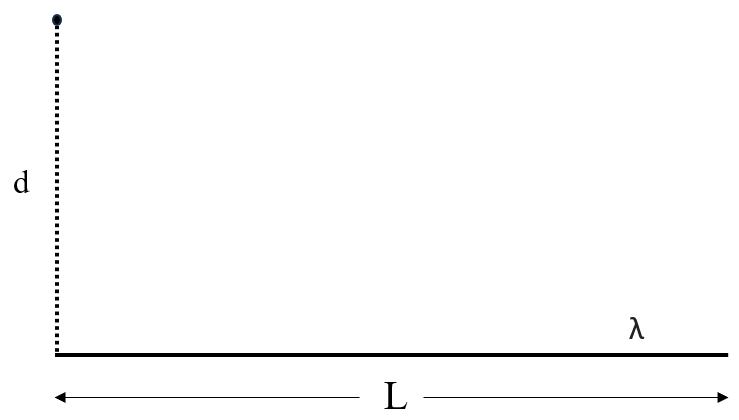
\includegraphics[width=0.5\textwidth]{EMq3figure.PNG}
    \caption*{}
\end{figure}

Find the electric field a distance, \( d \), above one end of a straight line segment of length \( L \) that has a constant line charge density \( \lambda \) (as seen in the figure). In the limit of \( d \gg L \), what does the electric field reduce to and what is its physical interpretation? \\

Q4. 

\begin{figure}[t]
    \centering
    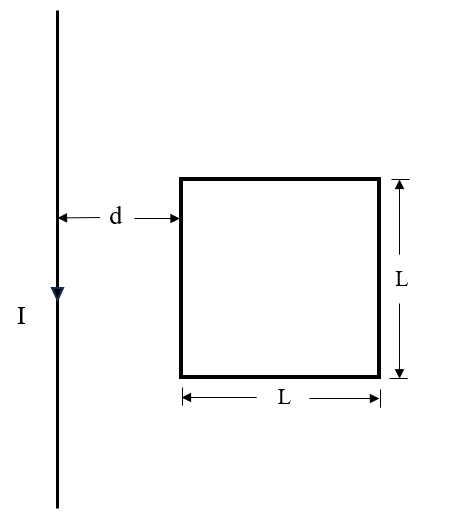
\includegraphics[width=0.4\textwidth]{EMq4figure.PNG}
    \caption*{}
\end{figure}

A square loop of wire (sides of length \( L \)) lies a fixed distance \( d \) from a very long straight wire, which carries a constant current \( I \) directed downwards (as seen in the figure).

\medskip

a) Find the flux of \( \underline{B} \) through the loop.

\medskip

b) If the loop is moved directly away from the wire to the right, at speed \( v \), what emf is generated? In what direction (clockwise or counterclockwise) does the current flow?

\medskip

c) What happens if the loop only moves downwards at speed \( v \)?

\newpage

Q5. 

Consider the circuit diagram seen in the figure. 

a) Calculate the current seen by the ammeter.

\medskip

b) Calculate the energy delivered by the \(12\, \text{V}\) battery in \(4\) seconds.

\begin{figure}[h!]
    \centering
    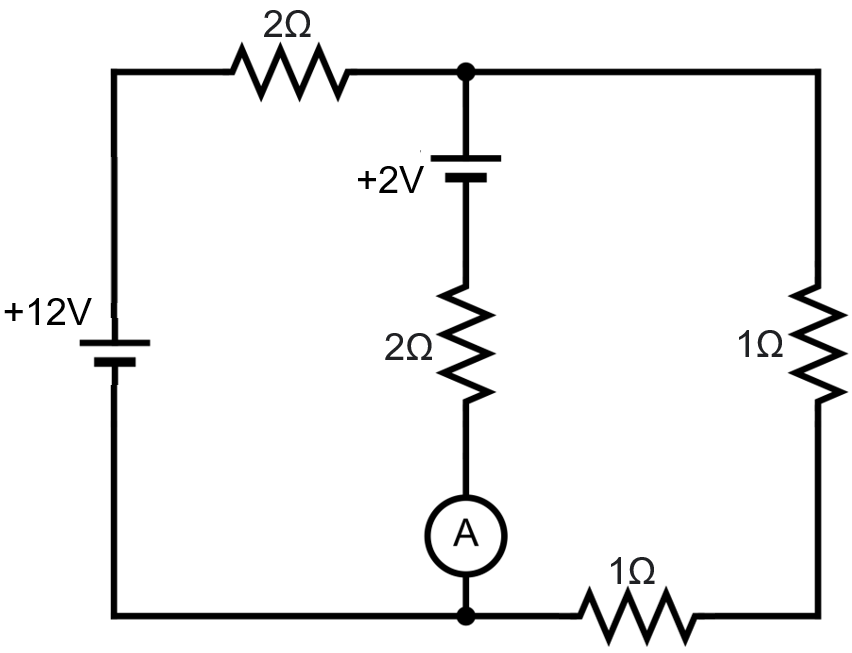
\includegraphics[width=0.5\textwidth]{EMq5figure.PNG}
    \caption*{}
\end{figure}

Q6. 

Two infinite parallel planes have equal and opposite uniform surface charge density \( -\sigma \) and \( +\sigma \), where \( \sigma \) is positive. The planes are separated by a distance of \( 15 \) cm, and the potential difference between the plates is \( 120 \) V.  

\medskip

a) Determine the electric field, \( \underline{E} \), between the plates.

\medskip

b) An object with charge \( +0.001 \, \text{C} \) and a mass of \( 23 \, \text{g} \) is held at rest at the positive plate, then let go. Determine the acceleration of the object. \\

Q7. 

An RLC circuit has a resistor with resistance \( R = 600 \, \Omega \), capacitor with capacitance \( C = 1500 \, \text{pF} \), inductor with inductance \( L = 20 \, \text{mH} \).

\medskip

a) What is the resonant frequency, \( \omega_{0} \), of the circuit?

\medskip

b) The circuit is driven with an e.m.f source of the form 

\[ \mathcal{E} = \mathcal{E}_{0} \cos(\omega t) \]

Find an expression for the voltage drop across the inductor, \( \Delta V_{L} \), as a function of \( \mathcal{E}_{0} \), the impedance \( Z \), inductive reactance \( X_{L} \), angular frequency \( \omega \), and some phase shift \( \phi \).

\medskip

c) Describe the phase relationship between the source e.m.f and voltage across the inductor in the limits of low frequency (\( \omega \ll \omega_{0} \)) and high frequency (\( \omega \gg \omega_{0} \)).

\bigskip

Q8. 

Two linear magnetic media occupy the half-spaces above and below the \( xy \) plane. The space \( z > 0 \) is occupied by Material 1, with relative permeability \( \mu_{r1} = 1.493 \). The magnetic field \( \underline{B}_{1} \) in this region is spatially uniform and static, with positive \( x \) and \( z \) components, and zero \( y \) component. It is directed at an angle \( \alpha_{1} \) with respect to the positive \( z \) direction. The space \( z < 0 \) is occupied by Material 2, with relative permeability \( \mu_{r2}= 3.012 \). The magnetic field \( \underline{B}_{2} \) in this region is spatially uniform and static, with positive \( x \) and \( z \) components, and zero \( y \) component. It is directed at an angle of \( \alpha_{2} = 45^\circ \) with respect to the positive \( z \) direction. There is no free current flowing anywhere in the system. Using the information above, calculate the value of the angle \( \alpha_{1} \). 

\bigskip

Q9. 

A transverse electromagnetic wave propagating in vacuum has an electric field which has complex representation:

\[ \underline{E}(\underline{r}, t) = \underline{E}_{0} \exp (i(\underline{k} \cdot \underline{r} - \omega t)) \]

With real valued vectors \( \underline{E}_{0} \), \( \underline{k} \).

\medskip 

a) Apply Faraday’s Law and show magnetic intensity of the wave has magnitude given by 

\[ H(\underline{r}, t) = \sqrt{\frac{\epsilon_{0}}{\mu_{0}}} E(\underline{r}, t) \]

\medskip

b) Show the Poynting flux averaged over one period of oscillation is given by 

\[ \left< \underline{N} \right> = \frac{1}{2} \sqrt{\frac{\mu_{0}}{\epsilon_{0}}} (H_{0})^{2} \hat{\underline{k}} \]

where \( H_{0} \) denotes the amplitude of the magnetic intensity.

c) The pressure exerted by radiation has intensity \( I \) on a perfect planar reflector has the value \( \frac{2I}{c} \), where \( c \) is the speed of light. Show that when the angle of incidence of radiation is \( \alpha \), the radiation pressure becomes \( 2I\cos^{2}{\alpha}/{c} \).\\

Q10. 

Consider 2 inertial reference frames \( S \) and \( S' \). The frames are aligned in such a way that origins of both frames coincide at time zero within both frames (\( t = t' = 0 \)). The frame \( S' \) moves with velocity \( v \) in the \( x \) direction as seen by \( S \). The transformation of electric and magnetic fields from frame \( S \) to \( S' \) is given by 

\[
\begin{aligned}
E'_{x} &= E_{x}, & E'_{y} &= \gamma(E_{y} - vB_{z}), & E'_{z} &= \gamma(E_{z} + vB_{y}) \\
B'_{x} &= B_{x}, & B'_{y} &= \gamma(B_{y} + \frac{v}{c^{2}} E_{z}), & B'_{z} &= \gamma(B_{z} - \frac{v}{c^{2}} E_{y})
\end{aligned}
\]

\medskip

a) Using the transformations given, show that the scalar product, \( (\underline{E} \cdot \underline{B}) \), is invariant under transformation.

\medskip

b) A plane electromagnetic wave observed in the reference frame \( S \) propagates in a vacuum along the \( x \) direction. In frame \( S \), it is represented by the Cartesian representation: 

\[ \underline{E} = E_{0} \hat{\underline{y}} \exp(i(kx - \omega t)) \]

with \( E_{0} \), a real value denoting the amplitude, \( k \) is the wavevector, and \( \omega \) the angular frequency. \( (kx - \omega t) \) defines the phase of the wave in frame \( S \). Show that this phase in reference frame \( S' \) is written \( (k'x' - \omega' t') \), where primed coordinates correspond to the frame \( S' \) and

\[ \omega' = \gamma(\omega - kv), \quad k' = \gamma(k - \frac{\omega v}{c^{2}}) \]

\medskip

c) Examine the relationship between the wave frequencies \( \omega \) and \( \omega' \) in the limit \( v/c \) approaches \( 0 \). What physical phenomenon does this represent? Justify your answer.

\newpage

\section{Quantum Mechanics}

Q1. Worded:

a) Define the commutator of 2 operators, \( \hat{P} \) and \( \hat{Q} \). Define what it means if \( \hat{P} \) and \( \hat{Q} \) are compatible operators. Explain what does compatibility imply about their commutator?

\medskip

b) Suppose that \( \hat{P} \) and \( \hat{Q} \) are not compatible. For a given system, \( \hat{P} \) is first measured giving a value \( p \), then \( \hat{Q} \) is measured giving the value \( q \). If \( \hat{P} \) is then measured again, what can be said about the possible results of the measurement and why? \\

Q2. Worded:

a) Quantum mechanical operators are Hermitian. What mathematical property do the eigenvalues of a Hermitian operator have? What is the physical interpretation of its eigenvalues?

\medskip

b) Explain what is meant if it is stated that the set of eigenfunctions \( \{ \phi_{n} \} \) of a Hermitian operator is orthonormal. \\

Q3.

For one dimension, an operator \( \hat{Q} \) is Hermitian if and only if 

\[ \int_{-\infty}^{\infty} f^{*}\hat{Q}g \, dx = \int_{-\infty}^{\infty} g(\hat{Q}f)^{*} \, dx \]

where \( f(x) \), \( g(x) \) are well-behaved functions which vanish at infinity, \( ^{*} \) denotes the complex conjugate. 

\medskip

a) Use the definition above to determine whether \( \hat{p} = -i\hbar\frac{d}{dx} \) is a Hermitian operator 

\medskip

b) Determine whether \( \hat{Q} = \frac{d^{2}}{dx^{2}} \) is a Hermitian operator.

\bigskip

Q4. 

Let \( \hat{L_{x}} \) be the x-component of the angular momentum operator. Let \( \hat{X} \), \( \hat{Y} \), \( \hat{Z} \) be the x, y, z components of the position operator respectively and \( \hat{P_{x}} \), \( \hat{P_{y}} \), \( \hat{P_{z}} \)  be the x, y, z components of the momentum operator respectively. Derive the following commutator relations:

\medskip

a) \( \left[ \hat{L_{x}}, \hat{X} \right] = 0 \)

\medskip

b) \( \left[ \hat{L_{x}}, \hat{P_{x}} \right] = 0 \)

\medskip

c) \( \left[ \hat{L_{x}}, \hat{Y} \right] = i \hbar \hat{Z} \)

\medskip

d) \( \left[ \hat{L_{x}}, \hat{P_{y}} \right] = i \hbar \hat{P_{z}} \)

\medskip

e) \( \left[ \hat{L_{x}}, \hat{P}^{2} \right] = 0 \) \\

Q5. 

An infinite square well of length \( L \) can be defined mathematically by the potential,

\[ V(x) = \begin{cases}
0 & \text{for } 0 \leq x \leq L,\\
+\infty  & \text{otherwise,} 
\end{cases} \]

A particle of mass \( m \) in the well has eigenfunctions

\[ \phi_{n}(x) = \sqrt{\frac{2}{L}} \sin\left(\frac{n \pi x}{L} \right) \]

with corresponding energy eigenvalues 

\[ E_{n} = \frac{n^{2}\hbar^{2}\pi^{2}}{2mL^{2}} \]

a) Calculate the first-order correction to the ground state energy if the system is perturbed by 

\[ \hat{H}' = V_{0} \sin\left(\frac{2 \pi x}{L} \right) \]

\medskip

b) Calculate and derive an expression for the first-order correction to all energy eigenvalues given that the system is perturbed by 

\[ \hat{H}' = L\alpha \delta\left(x - \frac{L}{2} \right) \]

where \( \alpha \) is a constant and \( \delta \) is the Dirac delta function.\\ 

Q6. 

Let \( \hat{\underline{L}} \) and \( \hat{\underline{S}} \) be the angular momentum and spin angular momentum quantum operators. 

\medskip

a) Given that \( \hat{\underline{J}} = \hat{\underline{L}} + \hat{\underline{S}} \), show that 
\[ \hat{J^{2}} =  \hat{L^{2}} + \hat{S^{2}} + \hat{L}_{+}\hat{S}_{-} +  \hat{L}_{-}\hat{S}_{+} + 2\hat{L}_{z}\hat{S}_{z} \]

Where you may use  \( \hat{L}_{\pm} = \hat{L}_{x} \pm i\hat{L}_{y} \), and \( \hat{S}_{\pm} = \hat{S}_{x} \pm i\hat{S}_{y} \)

\medskip

b) consider the state \( \left|l, m; s, m_{s} \right> = \left|l, m \right>\left|s, m_{s} \right> \). Here \( l \) is a quantum number of \( \hat{L^{2}} \), \( m \) is a quantum number of \( \hat{L}_{z} \). \( s \) is a quantum number of \( \hat{S^{2}} \) and \( m_{s} \) is a quantum number of \( \hat{S}_{z} \). Show that the state \( \left|l, -l; s, -s \right> \) is an eigenvector of \( \hat{J^{2}} \) and the corresponding eigenvalue. 

\medskip

c) Now consider an operator \( \hat{O} = a\hat{L^{2}} + b\hat{S}_{+}\hat{L}_{z} \). Where \( a \), \( b \) are constants

You are given the following result:
\[ \hat{S}_{+} \left|s, m_{s} \right> = \hbar \sqrt{s(s+1) - m_{s}(m_{s}+1)} \left|s, m_{s}+1 \right> \]

\smallskip

Find the matrix representation of \( \hat{O} \) for a chosen basis of kets \( \left|l=1, m; s=\frac{1}{2}, m_{s} \right> \)

\bigskip

Q7.

A beam of particles each of mass \( m \) moves in a space with potential energy \( V(x) = 0 \), described by the wavefunction \( \psi(x) = Ae^{ikx} \).

\medskip

a) What is the corresponding time-dependent solution \( \Psi(x,t) \)? Show that the probability per unit length of finding a particle is independent of both space and time.

\medskip

b) Evaluate the particle flux 

\[ \Gamma = -\frac{i\hbar}{2m}\left[ \Psi^{*}\frac{\partial\Psi}{\partial x} - \Psi\frac{\partial\Psi^{*}}{\partial x} \right] \]

for the state \( \Psi \), giving a physical interpretation of the result in terms of the velocity of the particles. \\

Q8.


The expectation of an operator \( \hat{Q} \) in one dimension can be written 

\[ \left< \hat{Q} \right> = \int_{-\infty}^{\infty} \Psi^{*}(x) \hat{Q} \Psi(x) \, dx \]

\medskip

a) For an operator \( \hat{Q} \) which does not vary with time, show the rate of change with time of the expectation value of \( \hat{Q} \) can be written

\[ \frac{d}{dt}\left<\hat{Q}\right> = \frac{1}{i\hbar}\left< \left[ \hat{Q}, \hat{H} \right] \right> \]

where \( \hat{H} \) is the Hamiltonian operator.  

\medskip

b) A particle of mass \( m \) is subject to a time-independent potential \( V(x) \). By evaluating \( \left[ \hat{X}, \hat{H}\right] \), where \( \hat{X} \) is the position operator, show that 

\[ m\frac{d}{dt}\left<\hat{X}\right> = \left<\hat{P}\right> \]

You may use the additional information: 

Time-dependent Schrödinger equation:
\[ \frac{\partial\Psi}{\partial t} = \frac{1}{i\hbar}\hat{H}\Psi \] \\

\medskip

Q9. 

Consider a beam of particles each of mass \( m \) with energy \( E > 0 \) incident from the left, subject to a one-dimensional potential step defined by

\[ V(x) = \begin{cases}
0 & \text{for } x \leq 0,\\
-V_{0}  & \text{for } x > 0 
\end{cases} \]

a) Show that \( \psi_{1}(x) = e^{ik_{1}x} + Be^{-ik_{1}x} \) is the general solution in the region \( x \leq 0 \) and \( \psi_{2}(x) = Ce^{ik_{2}x} \) is the general solution in the region \( x > 0 \), where \( B \) and \( C \) are constants. Define \( k_{1} \), \( k_{2} \) as part of your answer.

b) By applying appropriate boundary conditions, show that 

\[ C = \frac{2k_{1}}{k_{1}+k_{2}} \] and \[ B = \frac{k_{1}-k_{2}}{k_{1}+k_{2}} \]

c) Calculate the incident, reflected, and transmitted flux for this scattering potential and derive that the probability for transmission, \( T \), and the probability for reflection, \( R \), are given by 

\[ T = \frac{4k_{1}k_{2}}{(k_{1}+k_{2})^{2}} \]

\[ R = \frac{(k_{1}-k_{2})^{2}}{(k_{1}+k_{2})^{2}} \]

You may use that the particle flux for a particle beam is given by 

\[ \Gamma(x) = -\frac{i\hbar}{2m} \left(\psi^{*}\frac{d\psi}{dx} - \psi\frac{d\psi^{*}}{dx} \right) \]

Q10.

Consider the system of a quantum harmonic oscillator with eigenstates written \( \left| n \right> \) and corresponding eigenvalues \( E_{n} = \hbar\omega(n+\frac{1}{2}) \).

You are given the raising and lower operators \( \hat{a}_{\pm} \) defined by:

\[ \hat{a}_{\pm} = \frac{1}{\sqrt{2}}(\alpha \hat{x} \mp \frac{i}{\hbar\alpha} \hat{p}) \]

\[ \alpha = \sqrt{\frac{m\omega}{\hbar}} \]

where \( \hat{x} \), \( \hat{p} \) are the one-dimensional position and momentum operators respectively.

\medskip

a) Normalize the state \( \left| \psi \right> =  \left| 0 \right> + b \left| 1 \right> \) and calculate the expectation value of the Hamiltonian for \( \left| \psi \right> \). \( b \) is a constant.

\medskip

b) A perturbation of the form \( \hat{H}' = q \mathcal{E} \hat{x} \) is introduced to the system, where \( \hat{x} \) is the one-dimensional position operator. Rewrite the perturbation in terms of raising and lowering operators \( \hat{a}_{\pm} \).

\medskip

c) By applying the variational principle, show that using \( \left| \psi \right> \) as a trial state, the value of \( b \) which minimizes energy is 

\[ b = \frac{E_{1} - E_{0}}{g} - \sqrt{\frac{(E_{1} - E_{0})^{2}}{g^{2}} -1} \]

where \( g = \sqrt{2} q \mathcal{E} / {\alpha} \)

\section{Classical Mechanics}

Q1. Worded:

Define what is a conservative force in the context of classical mechanics. For a conservative force \( \underline{F} \), mathematically define the potential energy. Why is it not possible to define a potential energy for a force which is not conservative? \\

Q2. Worded:

The damped harmonic oscillator is governed by an equation of motion

\[
\frac{d^{2}x}{dt^{2}} + b\frac{dx}{dt}+kx=0
\]

State the 3 cases of damping and qualitatively describe the behavior of each case. \\

Q3. 

Two objects of masses \( m_{1} \) and \( m_{2} \) are separated by a distance \( d \). The object of mass \( m_{1} \) is at position \( \underline{r_{1}} \) and the object of mass \( m_{2} \) is at position \( \underline{r_{2}} \).

\medskip

a) Starting from the definition of center of mass, show that its position vector can be given by 

\[ \underline{R} = (1-k)\underline{r_{1}} + k\underline{r_{2}} \]

and find the appropriate value of \( k \). 

\medskip

b) Show that the center of mass lies on a line connecting the 2 masses and its distance from the 2 masses are \( d m_{2}/(m_{1}+m_{2}) \) from \( \underline{r_{1}} \) and \( d m_{1}/(m_{1}+m_{2}) \) from \( \underline{r_{2}} \). \\

Q4. 

In 2D polar coordinates, the velocity, \( \underline{v} \), and acceleration, \( \underline{a} \), are given by 

\[ 
\underline{v} = \dot{r} \underline{\hat{r}} + r \dot{\theta} \underline{\hat{\theta}} 
\]
\[ 
\underline{a} = (\ddot{r} - r \dot{\theta}^{2}) \underline{\hat{r}} + (r \ddot{\theta} + 2\dot{r}\dot{\theta} ) \underline{\hat{\theta}} 
\]

A particle of mass, \( m \), rotates with angular frequency, \( \dot{\theta} \), dependent on time and has radial velocity given by \( \dot{r} = - \gamma \), where \( \gamma \) is a constant. At time \( t = 0 \), the particle has radial position \( r_{0} \) and \( \dot{\theta} = \delta \). 

\medskip

a) Assuming angular momentum is conserved, derive an expression for the angular frequency \( \dot{\theta} \). Write your answer in terms of \( r_{0} \), \( \gamma \), and \( \delta \).

\medskip

b) What is the angular component of the acceleration?

\medskip

c) Derive an expression for the kinetic energy of the particle and show that 

\[
\frac{dK}{dt} = \frac{m r_{0}^{4} \gamma \delta^{2}}{(r_{0} - \gamma t)^{3}}
\] \\

Q5. 

\begin{figure}[h!]
    \centering
    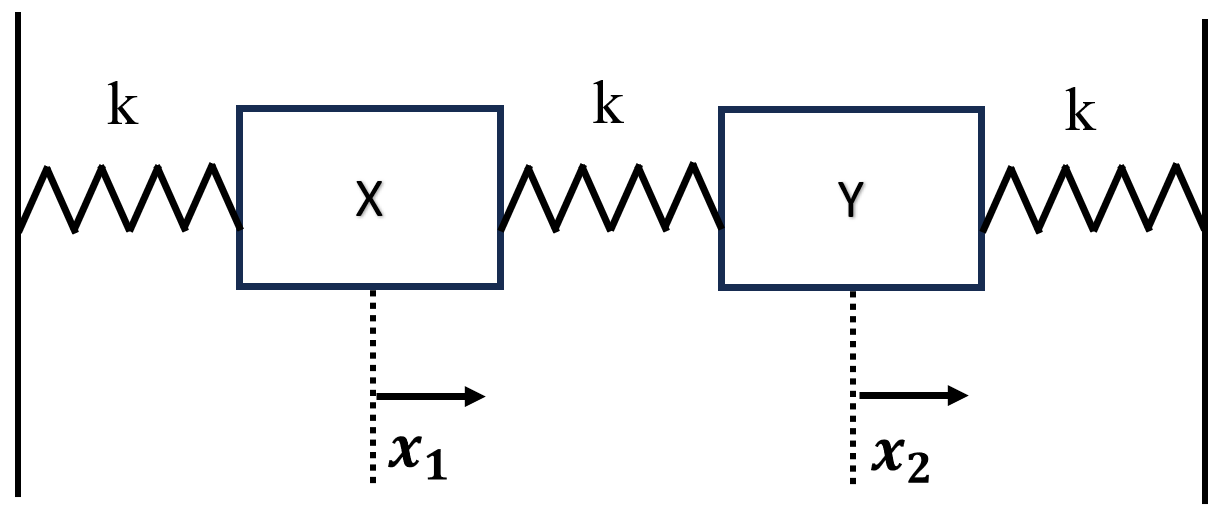
\includegraphics[width=0.5\textwidth]{CMq5figure.PNG}
    \caption*{}
\end{figure}

Two objects X and Y of the same mass, \( m \), are connected by a spring and each object is connected to a fixed wall by a spring (as seen in the figure). All springs have the same spring constant, \( k \). Initially object X is at rest whilst object Y moves with an initial velocity \( v \hat{\underline{i}} \). The horizontal displacement from equilibrium of X and Y is defined by \( x_{1} \) and \( x_{2} \) respectively. 

\medskip

a) Assuming no other forces besides those caused by the springs, derive the equations of motion for object X and object Y. 

\medskip

b) By defining new coordinates \( y_{1} = x_{1} + x_{2} \), \( y_{2} = x_{1} - x_{2} \), show that this uncouples the coordinates and \( y_{1} \) and \( y_{2} \) obey equations of undamped, undriven simple harmonic motion. 

\medskip

c) With the initial conditions of the system, show the solution of \( y_{1} \) is given by 

\[
y_{1} = v \sqrt{\frac{m}{k}} \sin(t \sqrt{\frac{k}{m}})
\]

Q6. 

Consider a Go-kart which moves around a flat circular track at a radius \( R \) with the track having a coefficient of static friction, \( \mu_{s} \). 

\medskip

a) Derive an expression for the largest speed the Go-kart can have whilst staying on the same circular path of radius \( R \). 

\medskip

b) Assume the track now forms an angle of \( \phi \) with respect to the horizontal flat ground and that the track is now frictionless. Rederive the largest speed the Go-kart may move with that maintains its circular motion around the track at the same radius \( R \). 

\medskip

c) Consider the same situation as in part b, except the static coefficient is now again \( \mu_{s} \). Derive the minimum speed, \( v_{min} \), and maximum speed, \( v_{max} \), showing that the following equality holds:

\[ 
v_{max}^{2} - v_{min}^{2} = \frac{2Rg\mu_{s}}{\cos^{2}(\phi) - \mu_{s}^{2}\sin^{2}(\phi)}
\]

Q7. 

a) State the form of the energy-momentum 4-vector of one particle of mass \( m \) and show that its scalar product is invariant under Lorentz transformation. In the lab frame, the particle moves with velocity \( \underline{v} \). 

\medskip

b) In its rest frame, the particle decays at rest into two identical massless particles which emerge along the positive and negative x-axis. Obtain expressions of the four-momenta of the two identical particles in the lab frame. 

\medskip

c) For \( m = 10 \) GeV/\( c^{2} \), \( \beta = v/c = 0.8 \), and if the two massless particles are photons, find their corresponding wavelengths in the rest frame of the decaying particle and in the lab frame. \\

Q8. 

\begin{figure}[h!]
    \centering
    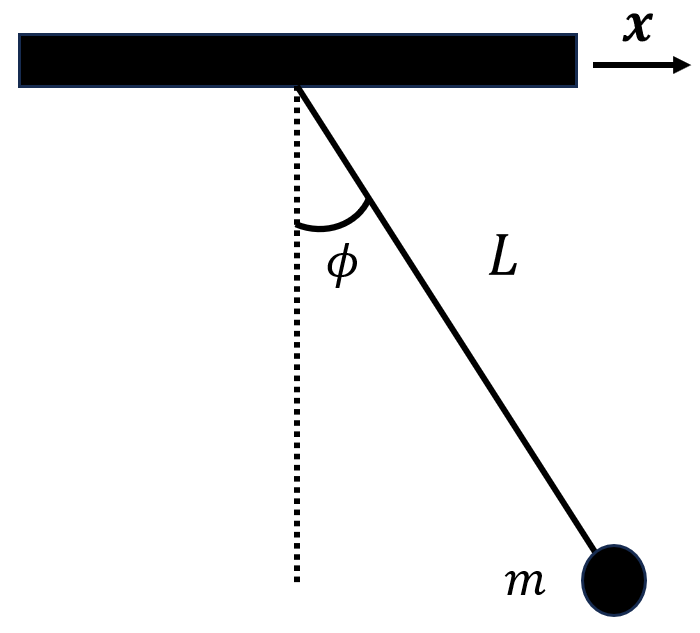
\includegraphics[width=0.5\textwidth]{CMq8figure.PNG}
    \caption*{}
\end{figure}

A pendulum under the influence of gravity is formed by a massless string of fixed length, \( L \), attached to a mass \( m \). The pendulum is connected to a support (as seen in the figure) which moves with a position given by 

\[ x(t) = v t^3 + A \sin(\omega t) \]

where \( v \) and \( A \) are constants.

\medskip

a) Starting from the expression of the Lagrangian, derive the equation of motion of the angle, \( \phi \), of the pendulum. 

\medskip

b) In the limit of \( v \), \(A\) approaching 0 and small angles (\( \phi \) approaching 0), show this reduces to the classic pendulum problem and equation of motion. \\

Q9. 

\begin{figure}[h!]
    \centering
    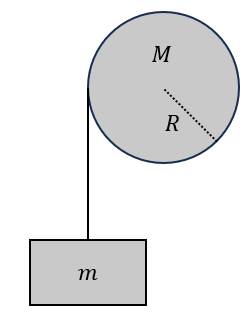
\includegraphics[width=0.3\textwidth]{CMq9figure.PNG}
    \caption*{}
\end{figure}

A rope connects to a block of mass \( m \) and wraps around a circular disk of mass \( M \) and radius \( R \). Due to gravity, the rope unwinds and the block falls down. 

\medskip

a) Derive expressions for the angular acceleration of the disk, the tension in the rope, and the acceleration of the block. Work under the assumption that the rope does not slip and that the moment of inertia of the disk is given by \( I = \frac{1}{2} m R^{2} \).

\medskip

b) Calculate the angular acceleration of the disk, tension in the rope, and acceleration of the block for the case \( m = 3 \) kg, \( M = 12 \) kg, \( R = 0.2 \) m. \\

Q10. 

On Earth, a ball of mass \( m \) is dropped from an airplane moving with horizontal velocity \( \underline{u} \). The air resistance on the ball causes a force opposite to the ball's velocity \( \underline{v} \), namely 

\[ \underline{F} = - b \underline{v} \] 

where \( b \) is a positive constant. 

\medskip

a) Using Newton's laws of motion, show that 
\[
m\frac{d\underline{v}}{dt} = - mg \hat{\underline{k}} - b\underline{v} 
\]

and show the solution to this equation is of the form 

\[
\underline{v} = \underline{A} e^{-bt/m} - \frac{mg}{b} \hat{\underline{k}} 
\]

where \( \underline{A} \) is a constant vector.

\medskip

b) Given that the ball initially starts with velocity \( \underline{u} \), find an expression for \( \underline{A} \).

\end{document}
